\documentclass[lettersize,journal]{IEEEtran}
\usepackage{amsmath,amsfonts}
\usepackage{algorithmic}
\usepackage{array}
\usepackage[caption=false,font=normalsize,labelfont=sf,textfont=sf]{subfig}
\usepackage{textcomp}
\usepackage{stfloats}
\usepackage{url}
\usepackage{verbatim}
\usepackage{graphicx}
\usepackage[UTF8]{ctex}

\usepackage{float}
\usepackage[justification=centering]{caption}

\usepackage{balance}
\begin{document}
\title{数据降维及可视化}
\author{姓名:尹伯豪\ 学号:2112215089}



\maketitle

\begin{abstract}
本文旨在阐述PCA算法的基本原理,并使用PCA算法和t-SNE算法对GTSRB数据集样本进行数据降维。同时,作者绘制了降维后的数据点空间分布图像,并对PCA与t-SNE算法进行了对比分析。此外,文章还对数据集中随机选取的一张图片进行了不同精度条件下的降维,并展示了其对比重构效果。
\end{abstract}



\section{PCA算法基本原理}

下面是几种常见聚类方法的公式:

1. K-means聚类方法:
   - 目标函数:
   
   $\arg\min_{\mathbf{C}} \sum_{i=1}^{n} \sum_{j=1}^{k} w_{ij} ||\mathbf{x}_i - \mathbf{c}_j||^2$
   
   - 公式说明:K-means聚类的目标是将数据集中的样本分为$k$个簇,每个簇的中心为$\mathbf{c}_j$,样本到簇中心的距离用欧氏距离$||\mathbf{x}_i - \mathbf{c}_j||^2$衡量,$w_{ij}$为二进制变量,表示样本$\mathbf{x}_i$是否属于簇$j$。

2. Mean Shift聚类方法:
   - 密度估计函数:
   
   $\hat{f}(x) = \frac{1}{nh^d} \sum_{i=1}^{n} K\left(\frac{x - x_i}{h}\right)$
   
   - 移动向量:
   
   $m(x) = \frac{\sum_{i=1}^{n} K\left(\frac{x - x_i}{h}\right) x_i}{\sum_{i=1}^{n} K\left(\frac{x - x_i}{h}\right)} - x$
   
   - 公式说明:Mean Shift聚类通过密度估计函数$\hat{f}(x)$计算样本$x$的密度,然后根据移动向量$m(x)$来更新样本的位置,直到收敛。聚类结果由收敛后的样本位置决定。

3. Spectral Clustering聚类方法:
   - 相似度矩阵:
   
   $W = (w_{ij})_{n \times n}$
   
   ,其中$w_{ij}$表示样本$x_i$和$x_j$之间的相似度。
   
   - 拉普拉斯矩阵:$L = D - W$,其中$D$是度矩阵。
   - 特征值分解:$L = U \Lambda U^T$,其中$U$是特征向量矩阵,$\Lambda$是特征值矩阵。
   - 公式说明:Spectral Clustering聚类方法通过计算相似度矩阵$W$和拉普拉斯矩阵$L$,然后进行特征值分解,得到特征向量矩阵$U$。最后,通过对特征向量进行聚类来得到最终的聚类结果。

这些公式描述了聚类方法的主要思想和数学原理,具体的实现细节可能有所差异,可以根据具体算法和论文进行详细了解。

PCA算法是一种常用的降维技术,其主要思想是将高维数据映射到低维空间中,以便于数据处理和可视化。其原理可以从不同的角度来解释,以下是三种常见的解释:

1. 最小化重构误差原理

PCA的第一种解释是最小化重构误差原理,即将高维数据映射到低维空间中,使得映射后的数据在重构回原始高维空间时误差最小。这个误差通常用重构误差或平方重构误差来度量,即原始数据与其在低维空间中的投影之间的距离平方和。

其主要思想是将数据投影到一个低维的子空间,使得在这个子空间中投影误差最小。具体来说,PCA通过对原始数据的协方差矩阵进行特征值分解,得到一组正交的基,这些基可以被用来表示原始数据的主要方向。将数据投影到这些基所构成的低维空间中,就可以得到一个新的低维表示,它最小化了重构误差,即从原始数据到低维表示再回到原始数据时的误差。

2. 最大化表示方差原理

PCA的第二种解释是最大化表示方差原理,即在低维空间中找到一个方向,使得在该方向上投影的数据方差最大。这个方向被称为第一主成分,它是数据方差最大的方向。我们可以将数据投影到这个方向上,从而得到一个一维的低维表示。接下来,我们可以找到第二主成分,即在与第一主成分正交的方向上投影的数据方差最大的方向。我们可以将数据投影到这个方向上,从而得到一个二维的低维表示。这个过程可以继续进行下去,直到我们得到所需的低维表示。

最大化表示方差原理的基本思想是,保留数据中最重要的方向,即方差最大的方向,以尽可能多地保留数据的信息。

3. 概率视角原理

PCA的第三种解释是概率视角原理,即将数据看作是由一个高维的潜在变量和一个高斯噪声组成的模型。PCA算法的目标是找到一个低维的表示,使得在这个低维表示下,潜在变量和噪声可以被分离开来。具体来说,我们可以假设潜在变量是低维的,且它们之间是独立的,而噪声是高斯分布的。通过对数据的协方差矩阵进行特征值分解,我们可以得到一组正交基,这些基可以被用来表示原始数据的主要方向,同时也对应着潜在变量的方向。因此,通过投影数据到这些基所构成的低维空间中,我们可以得到一个低维的表示,使得潜在变量可以被分离出来。

从概率视角看,PCA算法的优化目标是最大化数据的似然函数。具体来说,我们可以假设数据是由潜在变量和噪声组成的高斯混合模型,然后通过最大化数据的对数似然函数,即最大化观察到的数据在模型中的概率,来找到最佳的低维表示。在实际应用中,我们通常使用EM算法来估计模型参数,并得到最佳的低维表示。

\section{数据降维及可视化}

1. 数据预处理

在本次实验中,从GTSRB数据集中选择了10个类别,每个类别200张图片,共计2,000张图片。为了进行降维和可视化,对样本图像进行了简单预处理,将所有图像调整为相同的大小(32 x 32像素),并将其转换为灰度图像,以便降低计算复杂度和减少噪声。

2. 数据降维和可视化

使用sklearn.decomposition中封装的PCA算法保留前两个和前三个主成分,得到了2维和3维的降维结果。下图分别展示了2维和3维降维后的数据点在空间中的分布,每个数据点代表一张图片,不同的颜色代表不同的类别。

\begin{figure}[H]
\centering
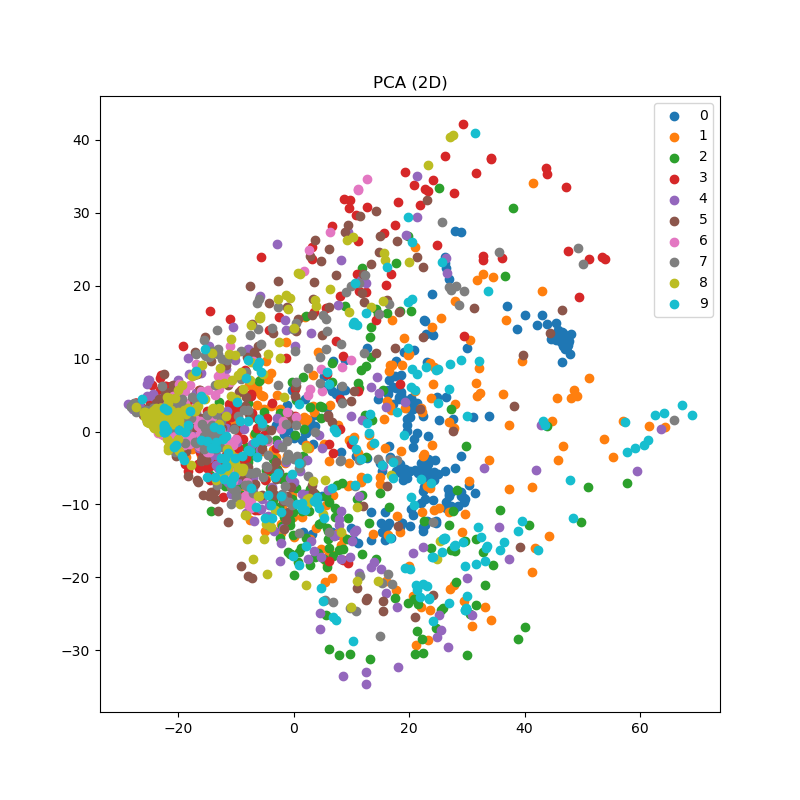
\includegraphics[width=2.5in]{image/Figure_1.png}
\caption{PCA降至2维数据点空间分布}
\end{figure}

\begin{figure}[H]
\centering
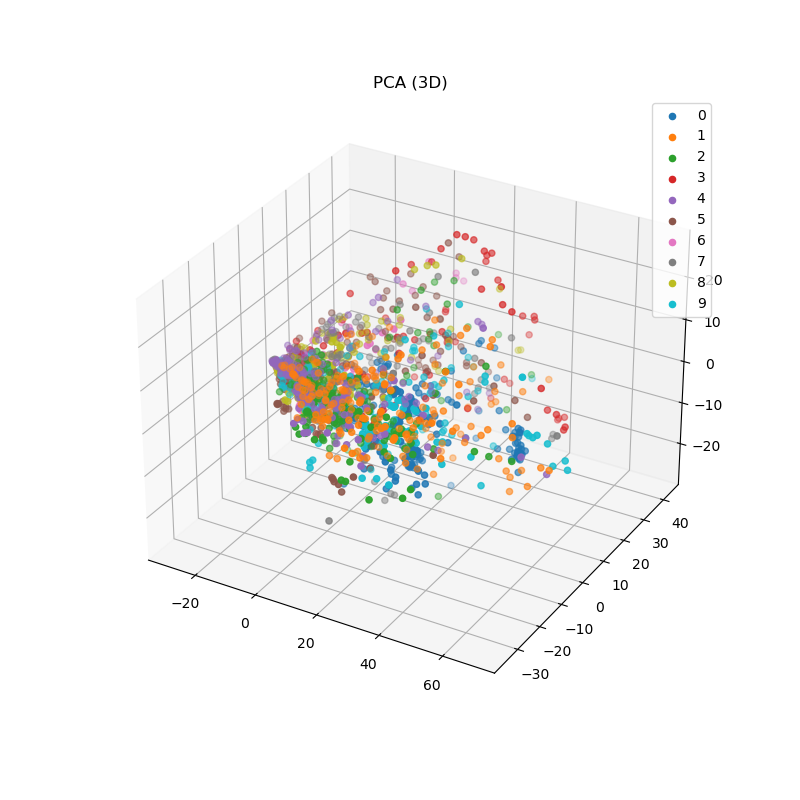
\includegraphics[width=2.5in]{image/Figure_3.png}
\caption{PCA降至3维数据点空间分布}
\end{figure}

从上图中可以看出,数据点在2D和3D空间中的分布呈现出一定的聚类趋势,且不同类别之间的差异性较大,这说明PCA方法可以在保留数据点间线性关系的同时,有效地将数据进行降维。

使用sklearn.manifold中的t-SNE方法对GTSRB数据集中同样的数据进行降维可视化,得到了2维和3维的降维结果,其中t-SNE模型的超参数设置了一些常见值。

\begin{figure}[H]
\centering
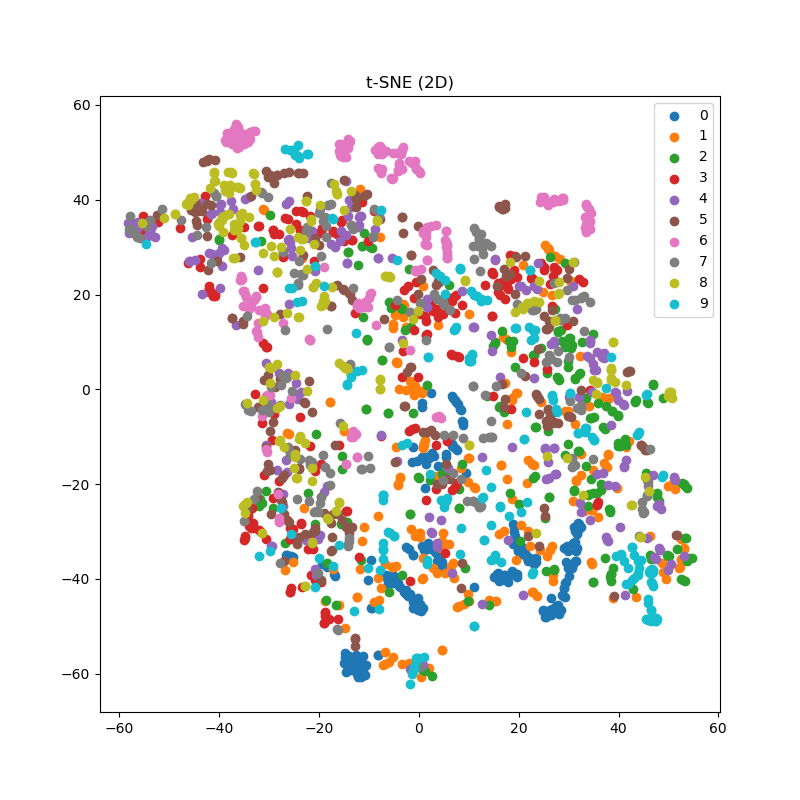
\includegraphics[width=2.5in]{image/Figure_2.png}
\caption{t-SNE降至2维数据点空间分布}
\end{figure}

\begin{figure}[H]
\centering
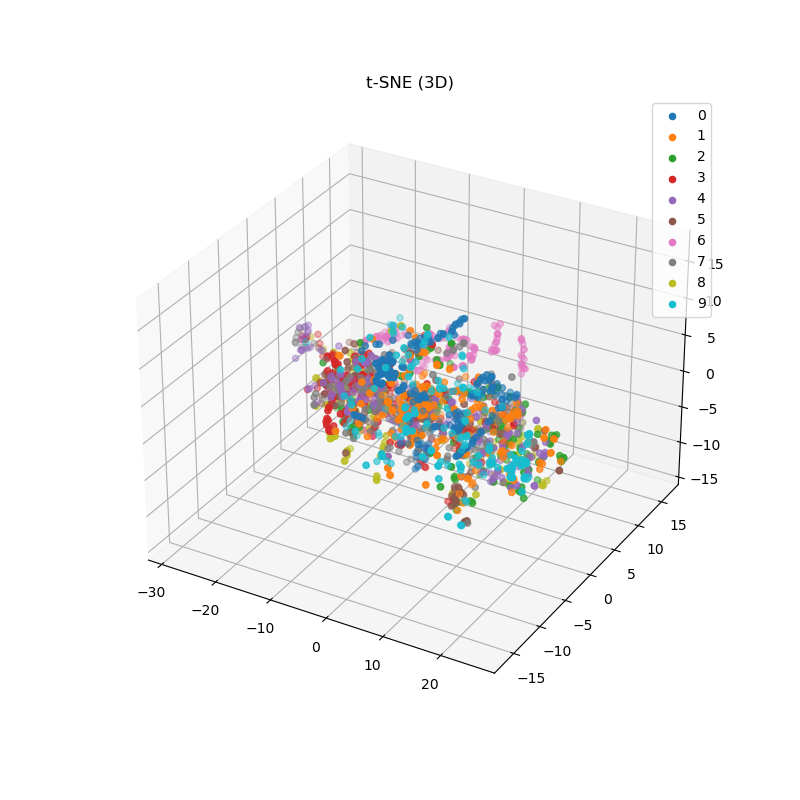
\includegraphics[width=2.5in]{image/Figure_4.png}
\caption{t-SNE降至3维数据点空间分布}
\end{figure}

从上图中可以看出,使用t-SNE方法降维和可视化数据点时,不同类别的数据点在2D和3D空间中都呈现出了明显的聚类趋势,且同一类别的数据点之间的距离相对较近。这说明,t-SNE方法能够在保留数据点间复杂非线性关系的同时,有效地将数据进行降维。

综上所述,通过结果的可视化展示,可以看出。t-SNE在降维后的数据点分布更加分散,不同类别之间的区分度更高,而PCA在降维后的数据点分布更加集中,但不同类别之间的区分度较低。并且t-SNE在降维时更加关注数据点之间的相似度,更加擅长发现高维空间中的局部结构,而PCA在降维时更加关注数据点的全局结构,更加擅长发现高维空间中的主要方向。在项目的运行中也发现t-SNE在降维时计算复杂度较高,需要耗费较长的时间和计算资源,而PCA计算速度较快。

\section{不同精度数据降维对比}

\begin{figure}[H]
\centering
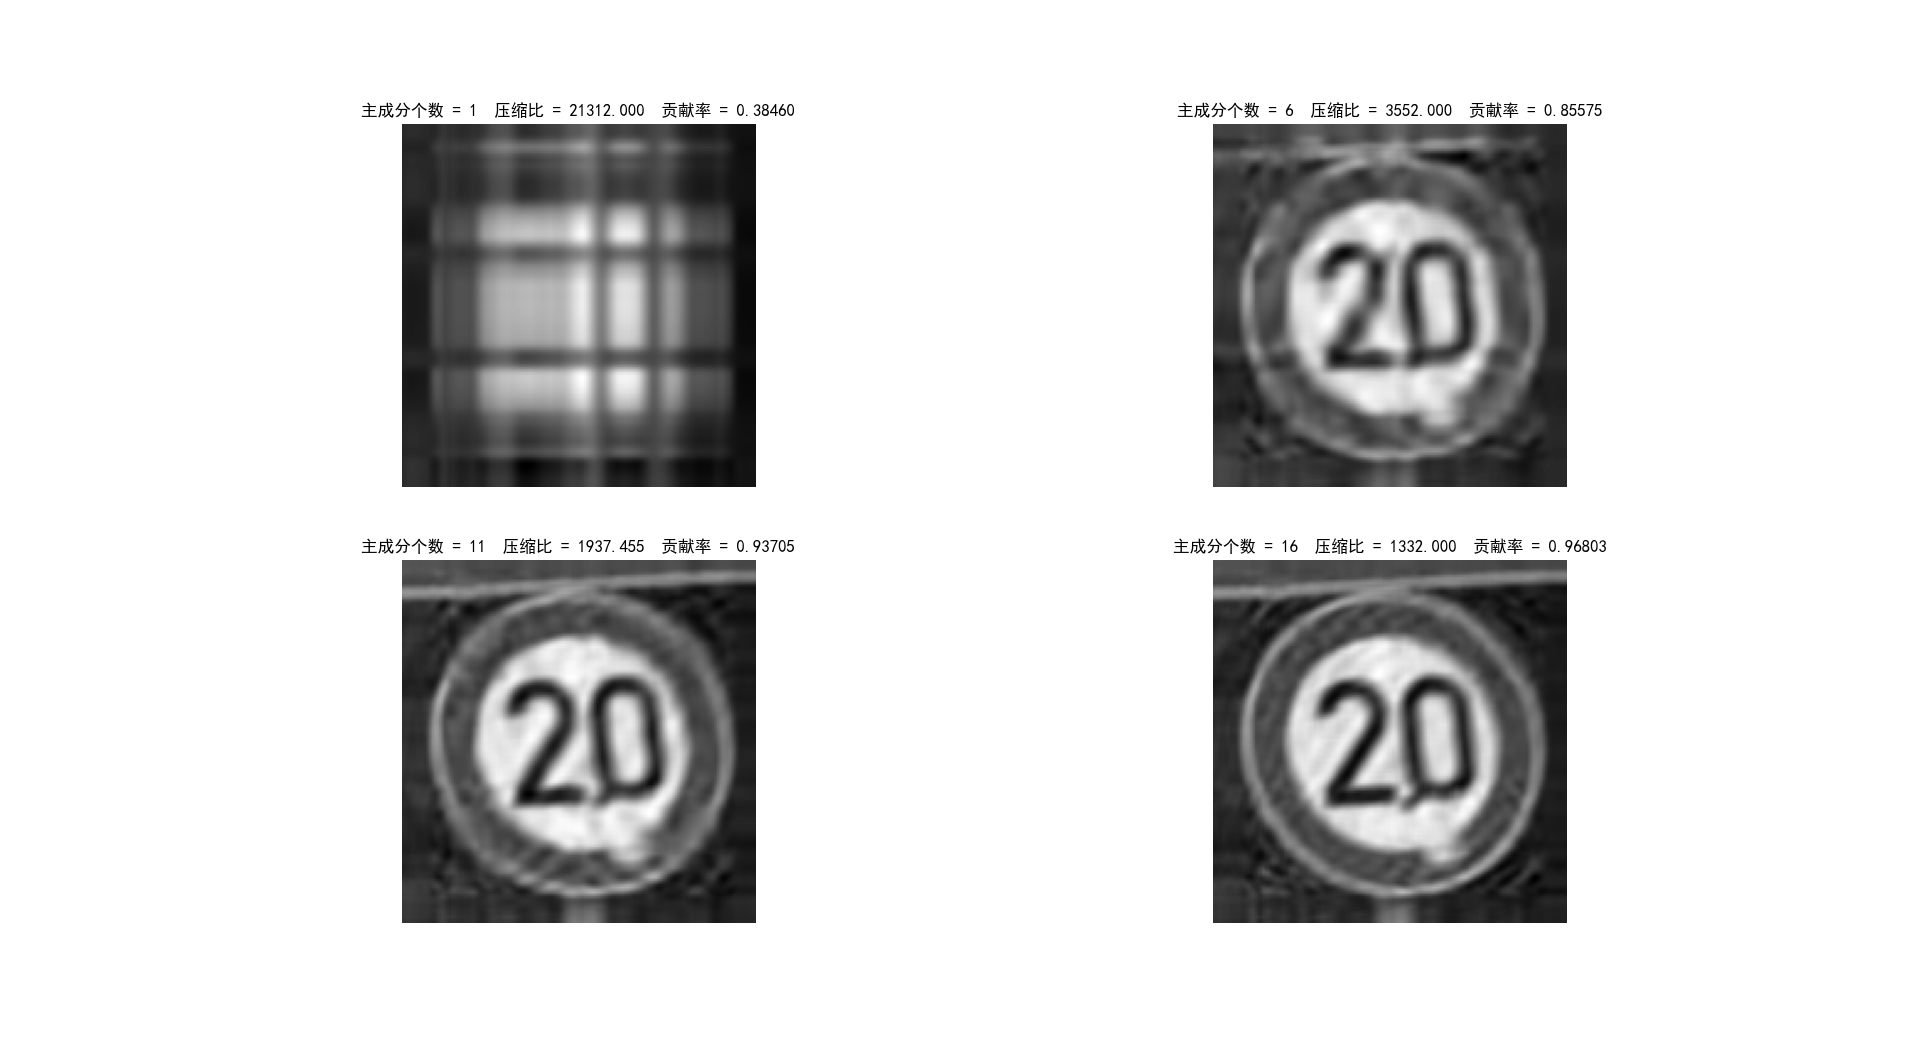
\includegraphics[width=3in]{image/Figure_6.png}
\caption{不同精度的降维效果}
\end{figure}

从输出图像可以看出,随着主成分个数的减少,降维后的图像逐渐失去了细节和清晰度,但整体仍能较好地保留原始图像的轮廓和结构。同时,压缩比随着主成分个数的减少而增加,说明在较少的主成分个数下,能够较大程度地压缩原始图像数据的体积。而贡献率则表示了保留了多少原始图像的信息,从中也可以看出降维后的图像质量的好坏。

\section{总结}

本次实验基于GTSRB数据集,分别使用PCA和t-SNE方法对其进行降维和可视化,并进行对比分析。实验结果表明,t-SNE方法相对于PCA方法具有更好的降维效果,在保留数据点间复杂非线性关系的同时,能够将数据点进行有效地聚类和分类。但是,t-SNE方法计算量较大,对于大规模数据集的处理可能存在一定的挑战。最后,通过本次实验,我了解了降维方法的基本原理和实际应用,以及不同降维方法的优缺点和适用范围,为后续的数据分析和处理的学习打下了基础。

\begin{thebibliography}{1}

\bibitem{ams}
{\it{数据降维—PCA}}, {\it{BCKou}}, {\it{CSDN}}, {\it{2022年10月10日}}, \url{https://blog.csdn.net/loser_k/article/details/124454794}

\bibitem{ams}
{\it{Pca,Kpca,TSNE降维非线性数据的效果展示与理论解释}}, {\it{时光之笛}}, {\it{知乎}}, {\it{2022年3月22日}}, \url{https://zhuanlan.zhihu.com/p/405398153}

\bibitem{ams}
{\it{机器学习--主成分分析(PCA)算法的原理及优缺点}}, {\it{泰初}}, {\it{CNBLOGS}}, {\it{2019年10月29日}}, \url{https://www.cnblogs.com/lsm-boke/p/11760224.html}

\bibitem{ams}
{\it{chatgpt}}, gpt-3.5-turbo API

\end{thebibliography}



\end{document}


